\begin{enumerate}[label=\thesubsection.\arabic*.,ref=\thesubsection.\theenumi]
\numberwithin{equation}{enumi}


\item The asymptotic Bode phase plot of 
%
\begin{align}
\label{eq:ee18btech11037_gs}
G(s) = \frac{k}{(s+0.1)(s+10)(s+{p_1})}
\end{align}
%
with k and $p_1$ both positive, is shown in Fig. \ref{fig:ee18btech11037}.  Express it as a piecewise linear function of $\log \brak{\omega}$.
\begin{figure}[!ht]
\centering
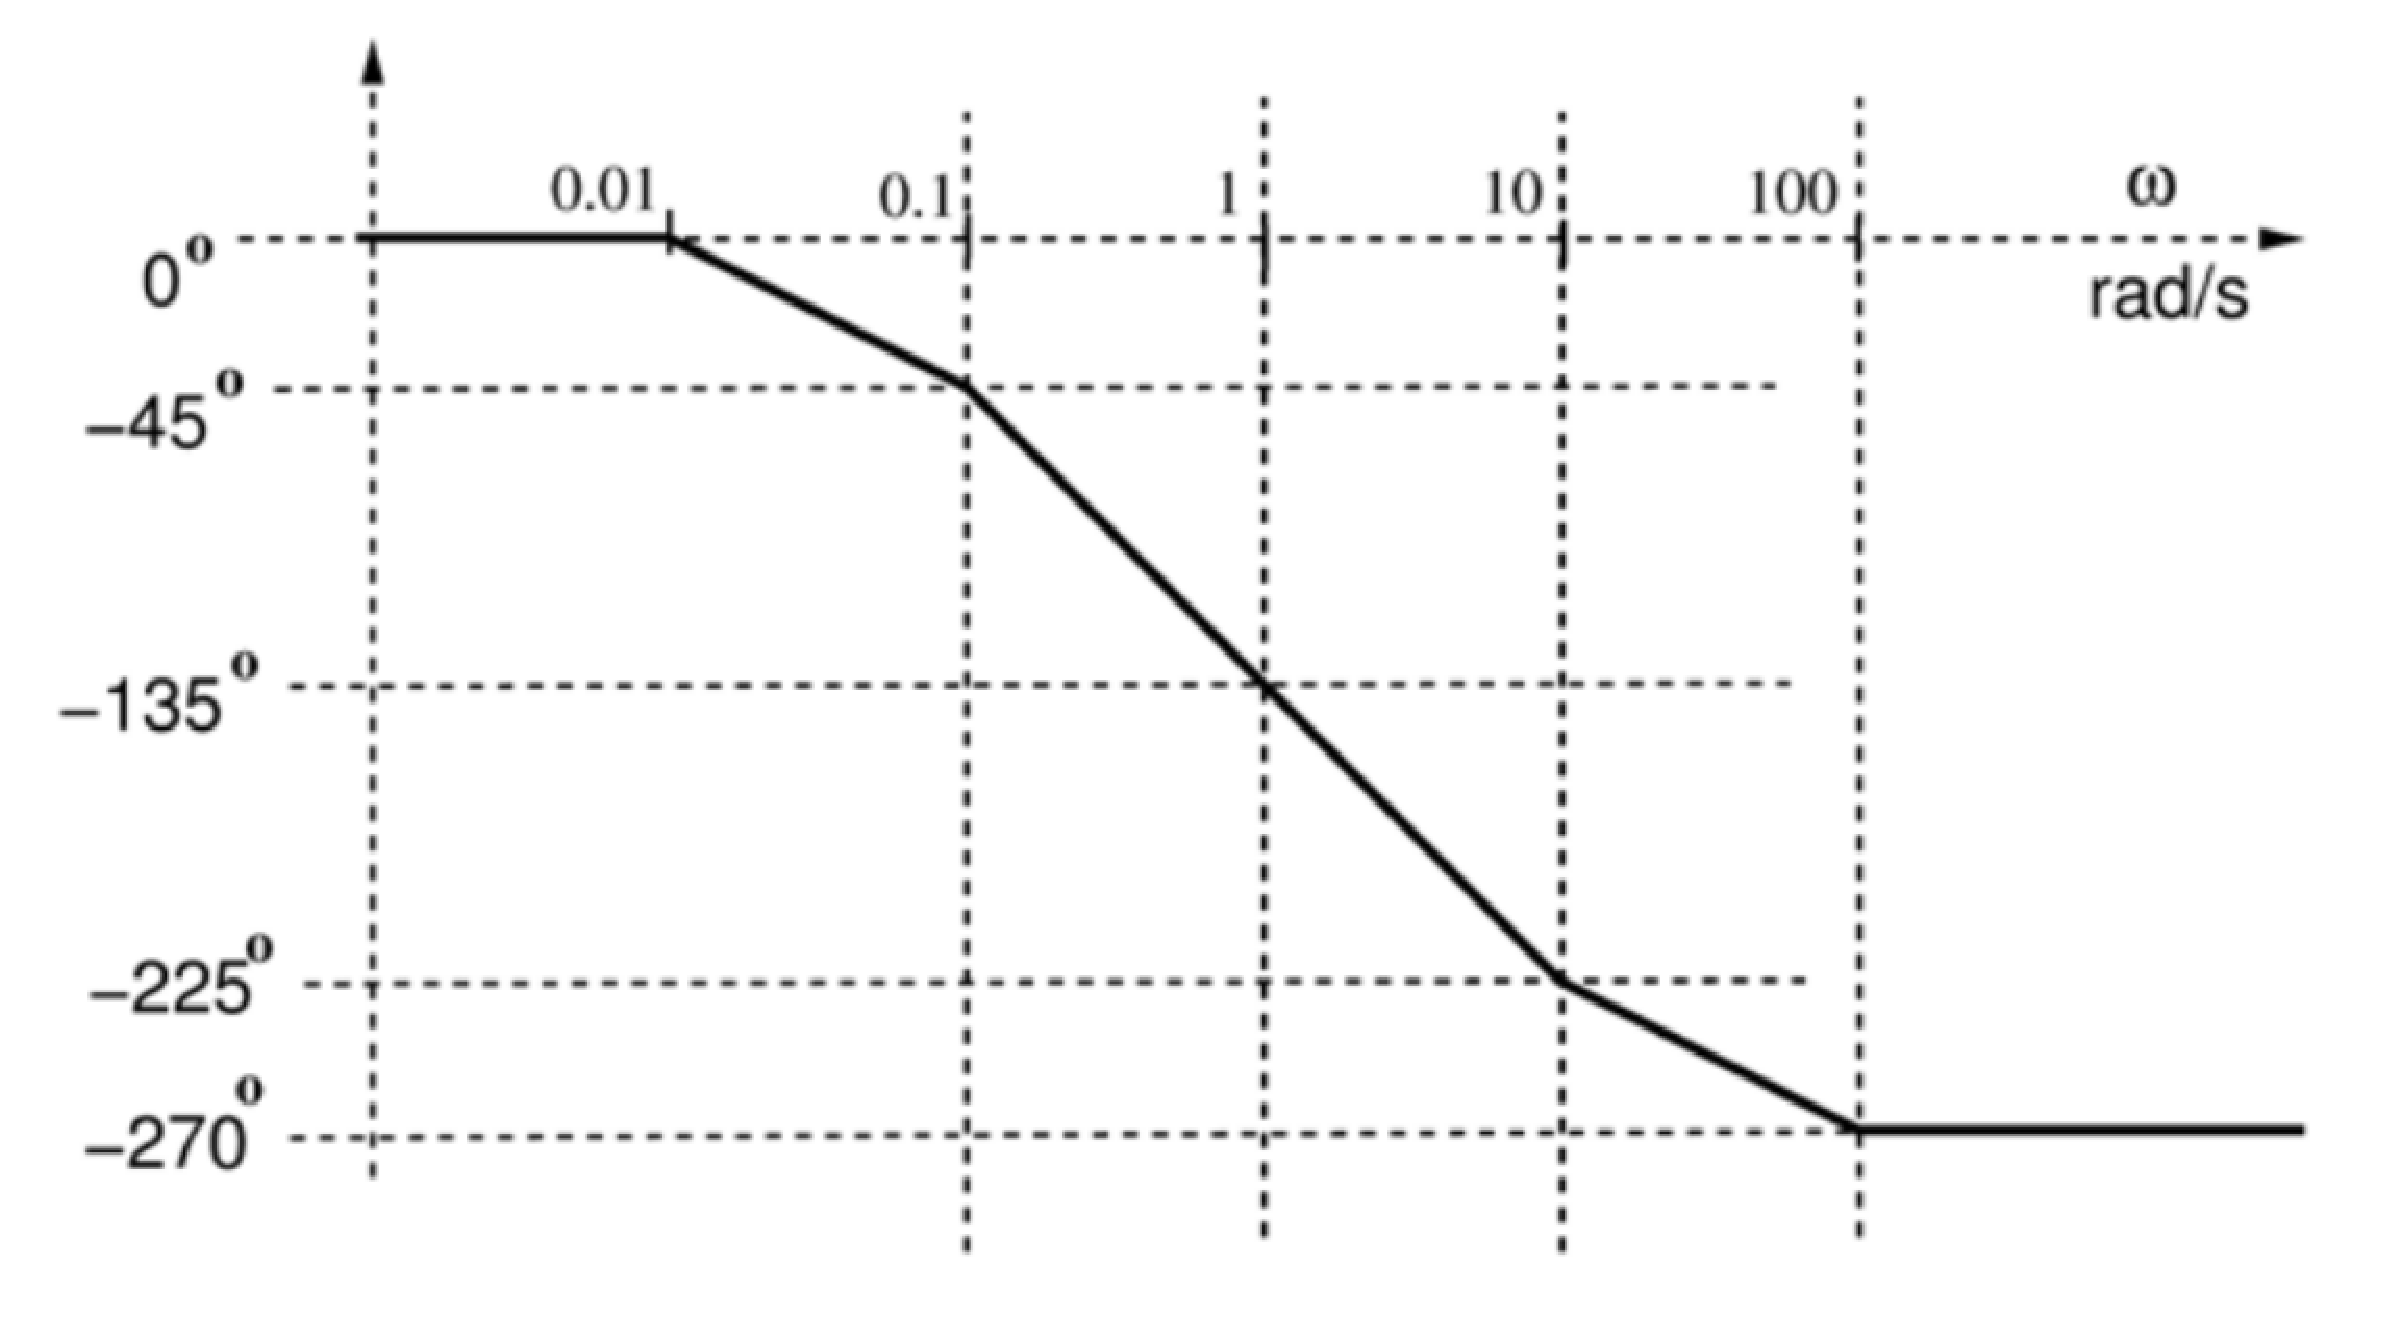
\includegraphics[width=\columnwidth]{./figs/ee18btech11037/ee18btech11037.eps}
\caption{}
\label{fig:ee18btech11037}
\end{figure}
\\
\solution The desired expression is
\begin{align}
\label{eq:ee18btech11037_totalphase}
 \phi(\omega) = 
 \begin{cases} 
        0 & 0<\omega<0.01 \\
      -90-45\log(\omega)& 0.01<\omega<0.1 \\
      -135-90\log(\omega)& 0.1<\omega<10 \\
      -180-45\log(\omega)& 10<\omega<100 \\
      -90 & 100<\omega  
 \end{cases}
\end{align}

\item Find  $p_1$.
\\
\solution 
%Bode phase plot for a transfer function having a single pole at $p_1$
Let 
\begin{align}
\label{eq:ee18btech11037_g1}
G_1(s) = \frac{1}{(s+{p_1})}
\end{align}
%
The equivalent Bode phase is
\begin{align}
\begin{split}
\label{eq:ee18btech11037_part1_of_phase}
 \phi _1(\omega) &= \angle G_1\brak{\j\omega}
\\
&= 
 \begin{cases} 
        0 & 0<\omega< \frac{p_1}{10} \\
      -45\times\brak{\log\brak{\frac{10\omega}{p_1}}}& \frac{p_1}{10}<\omega<10p_1 \\
      -90 & 10p_1<\omega  
 \end{cases}
\end{split}
\end{align}
%
Similarly, let
\begin{align}
\label{eq:ee18btech11037_g2}
G_2(s) = \frac{k}{(s+0.1)(s+10)}.
\end{align}
%
The equivalent Bode phase is
%
\begin{align}
\label{eq:ee18btech11037_part2_of_phase}
\begin{split}
 \phi_2(\omega) &=  \angle G_2\brak{\j\omega}
\\
&=
 \begin{cases} 
        0 & 0<\omega<0.01 \\
      -90-45\log(\omega)& 0.01<\omega<100 \\
      -180 & 100<\omega  
 \end{cases}.
\end{split}
\end{align}
Hence, from  \eqref{eq:ee18btech11037_part1_of_phase} and \eqref{eq:ee18btech11037_part2_of_phase},
\begin{align}
\phi(\omega) = \phi_1(\omega) + \phi_2(\omega) 
\end{align} 
From \eqref{eq:ee18btech11037_totalphase} and \eqref{eq:ee18btech11037_part2_of_phase}
\begin{align}
\phi(\omega) = \phi_2(\omega)  \quad   0<\omega<0.1 \\
\label{eq:ee18btech11037_phi1}
\implies \phi_1(\omega) = 0 \quad  0<\omega<0.1 
\end{align}
%
This is obvious from Figs. \ref{fig:ee18btech11037_2} and Fig. \ref{fig:ee18btech11037}.
%Comparing \eqref{eq:ee18btech11037_phi1} with \eqref{eq:ee18btech11037_part1_of_phase},
Thus,
\begin{align}
\frac{p_1}{10} = 0.1
\implies p_1 = 1
\end{align}
%
%shows the bode phase plots corresponding to the poles 0.1 and 10.
%Comparing the second subplot in Fig. \ref{fig:ee18btech11037_2} generated by
The following code generates Fig. \ref{fig:ee18btech11037_2}
%
\begin{lstlisting}
codes/ee18btech11037.py
\end{lstlisting}
%ith Fig. \ref{fig:ee18btech11037}, the graph remains same till 0.1 and after 0.1 slope of the line differs. So, the phase plot for \eqref{eq:ee18btech11037_g1} remains 0 till 0.1.
%
\begin{figure}[!ht]
\centering
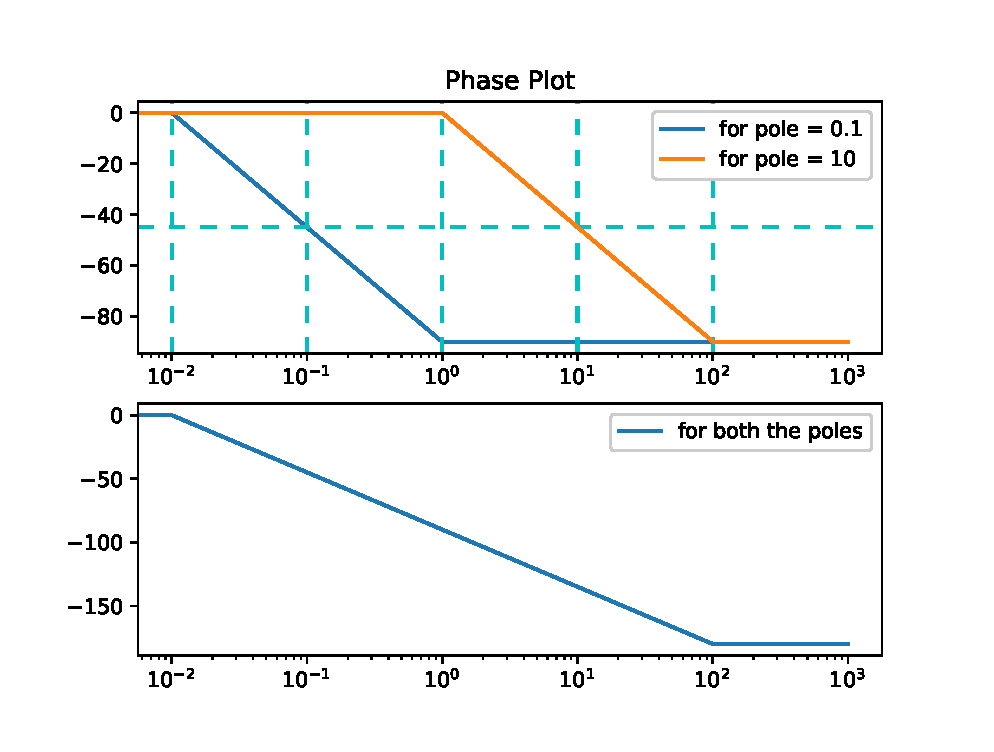
\includegraphics[width=\columnwidth]{./figs/ee18btech11037/ee18btech11037_2.eps}
\caption{}
\label{fig:ee18btech11037_2}
\end{figure}

\item Find the value of $p_1$ using phase of the transfer function.
\\
\solution
\begin{align}
\phi(\omega) = -\tan^{-1} \brak{\frac{\omega}{0.1}}-\tan^{-1} \brak{\frac{\omega}{10}}-\tan^{-1} \brak{\frac{\omega}{p_1}}
\end{align}
From the plot,
\begin{align}
-45\degree = -\tan^{-1}\brak{\frac{0.1}{0.1}} -\tan^{-1}\brak{\frac{0.1}{10}} -\tan^{-1}\brak{\frac{0.1}{p_1}}
\end{align}
 $p_1$ is approximately 1, i.e, for $p_1$ in 0.95 to 1.05 the $\phi$ is approximately equals to $-45\degree$.
%

\end{enumerate}
